\documentclass[11pt,spanish]{article}

% Paquetes
\usepackage{amstext}
\usepackage{amssymb}
\usepackage{amsmath}
\usepackage{babel}
    \addto\shorthandsspanish{\spanishdeactivate{~<>}}
    \decimalpoint
\usepackage[style=iso]{datetime2}
\usepackage{fancyhdr}
\usepackage{float}
\usepackage[T1]{fontenc}
\usepackage[a4paper]{geometry}
    \geometry{verbose,tmargin=3cm,bmargin=2cm,lmargin=2.5cm,rmargin=2.5cm}
\usepackage{graphicx}
\usepackage{hyperref}
\usepackage[utf8]{inputenc}
\usepackage{lastpage}
\usepackage{mathptmx}
\usepackage{tasks}
\usepackage{units}
\usepackage{siunitx}

% dibujos 

\usepackage{tikz}
\usepackage{tikz-dimline}
\usetikzlibrary{calc}
% \usetikzlibrary{math}
\usetikzlibrary{arrows.meta}
\usetikzlibrary{snakes}
\usetikzlibrary{decorations}
\usetikzlibrary{decorations.pathmorphing}
\usetikzlibrary{patterns}

% tipo de fuente 
\usepackage{lmodern}

\pagestyle{fancy}
\lfoot{\small DF, FCEyN, UBA}
\cfoot{\tiny Actualizado el {\today} a las {\DTMcurrenttime}}
\rfoot{\small Pág. {\thepage} de \pageref{LastPage}}

\begin{document}

% Título
    \begin{center}
    \textsc{\large Física 2 (Física) -- Cátedra Diego Arbó}
    \par\end{center}{\large \par}
    
    \begin{center}
    \textsc{\large Primer Cuatrimestre de 2025}
    \par\end{center}{\large \par}
    
    \begin{center}
    \textsc{\large Guía 9: Polarización}
    \par\end{center}{\large \par}

% Comienzo 
\begin{enumerate}


\section*{Estados de polarización}

% Ejercicio 1

    \item ¿Cuándo dos ondas transversales, perpendiculares entre sí, dan una
    onda:

    \begin{itemize}
        \item linealmente polarizada;
        \item circularmente polarizada en sentido antihorario;
        \item circularmente polarizada en sentido horario;
        \item elípticamente polarizada en sentido antihorario? 
    \end{itemize}
    
% Ejercicio 2    
    
    \item Escriba la expresión matemática de:

    \begin{enumerate}
        \item Una onda linealmente polarizada cuyo plano de polarización forma
        un ángulo de 30$^{\circ}$ con el eje $x$ (se propaga según el eje $z$).

        \item Una onda que se propaga según el eje $x$, polarizada circularmente
        en sentido horario.

        \item Una onda elípticamente polarizada en sentido horario, que se
        propaga según el eje $x$, tal que el eje mayor, que es igual a dos veces
        el eje menor, está sobre el eje $y$.

        \item Una onda elípticamente polarizada en sentido antihorario. La onda
        se propaga según el eje $x$ positivo (use terna directa). 
    \end{enumerate}

% Ejercicio 3

    \item Demuestre que siempre se puede describir una onda, cualquiera sea
    su polarización, como suma de dos ondas circularmente polarizadas
    en sentidos horario y antihorario.


\section*{Polarizadores lineales}

% Ejercicio 4

    \item Considere un haz de luz linealmente polarizada que incide sobre un
    polarizador lineal ideal. A continuación del polarizador se encuentra un
    detector de ley cuadrática.
    
    \begin{enumerate}
        \item Halle el vector campo eléctrico a la salida del polarizador en
        función del ángulo $\theta$ que forma el eje de transmisión con el campo
        eléctrico incidente, y analice su estado de polarización.
        
        \item Calcule la energía del campo eléctrico saliente en función de
        dicho ángulo y de la energía del haz incidente (ley de Malus).
        
        \item Grafique la ley de Malus y discuta cómo se modifica el gráfico si
        se elije un sistema de coordenadas diferente para medir los ángulos.
    \end{enumerate}
    
    \textbf{Sugerencia:} Elija el sistema de coordenadas más sencillo que le
    permita estudiar la dependencia según $\theta$ sin pérdida de generalidad. 

% Ejercicio 5

    \item Se reemplaza el haz de luz del ejercicio anterior por otro de luz
    circularmente polarizada derecha.
    
    \begin{enumerate}
        \item Halle el vector campo eléctrico a la salida del polarizador,
        verifique que corresponde a un estado de polarización lineal, y calcule
        su energía, en función de la inclinación del eje de transmisión del
        polarizador.
        
        \item Interprete físicamente el resultado obtenido y discuta si es
        posible definir la inclinación del eje de transmisión tomando como
        referencia al campo eléctrico incidente.
        
        \item ¿Qué cambia si se emplea un haz con el sentido de giro opuesto?
    \end{enumerate}

% Ejercicio 6

    \item Se reemplaza el haz de luz del ejercicio anterior por otro de luz
    elípticamente polarizada con sentido de giro arbitrario.
    
    \begin{enumerate}
        \item Repita los cálculos pedidos en los dos ejercicios anteriores, en
        función de la inclinación relativa entre el eje de transmisión del
        polarizador y alguno de los semiejes de la elipse que describe el haz
        incidente.
        
        \item Grafique la expresión para la intensidad saliente y analice bajo
        qué condiciones se recuperan los resultados obtenidos para luz circular
        y luz lineal. ¿Es posible extender la ley de Malus?
    \end{enumerate}
    
% Ejercicio 7

    \item Por último, se reemplaza el haz de luz del ejercicio anterior por otro
    de luz natural (también llamada polarización aleatoria). La misma puede
    describirse de la siguiente manera:
    
    $$\vec{E} = A(\hat{x} + e^{i \xi}\hat{y})$$
    
    donde $\xi$ es una variable aleatoria distribuída uniformemente en el
    intervalo $[0, 2 \pi)$.
    
    \begin{enumerate}
    
        \item Analice los posibles estados de polarización de un único pulso
        breve (duración $\sim 10^{-9}$ ns) emitido por dicha fuente, en función
        de $\xi$.
        
        \item Calcule la energía de cada pulso (promediada sobre un ciclo de
        oscilación) y la energía que mediría un detector expuesto a una sucesión
        infinita de dichos pulsos (promediada sobre muchos ciclos de
        oscilación). Compare ambas energías e interprete físicamente.
    
        \item Obtenga el campo eléctrico a la salida del polarizador, analice su
        estado de polarización, y calcule su intensidad promediando sobre un
        ciclo de oscilación. ¿De qué parámetros depende dicha intensidad?
        
        \item Discuta la necesidad de promediar la intensidad saliente obtenida
        sobre todos los estados posibles de luz incidente. ¿Cómo es el campo
        eléctrico que recibe el detector ubicado a la salida, para un tiempo $T$
        mucho mayor que el período de oscilación?
        
        \item Compare el perfil obtenido para la intensidad saliente con el caso
        estudiado anteriormente de luz circular. Interprete físicamente.
    \end{enumerate}

%    \item Incide un haz de luz natural de intensidad $I_{0}$ sobre un
%    polarizador lineal (ideal). ¿Qué intensidad se transmite? ¿Por qué?
    
%    \item Se hace incidir luz plano polarizada normalmente sobre un polarizador
%    lineal. Al ir rotando la lámina, ¿cómo varían el estado de polarización
%    y la intensidad del haz transmitido? Indique a partir de qué dirección
%    mide el ángulo de giro.

%    \item Sobre un polarizador incide una onda circularmente polarizada en
%    sentido horario. ¿Cuál es el estado de polarización de la onda transmitida?
%    ¿Qué fracción de la intensidad incidente se transmitió a través de
%    la lámina? Justifique.
    
% Ejercicio 8
    
    \item Sobre un polarizador lineal ideal incide una onda cuyo estado de
    polarización no se conoce, con una intensidad $I_{0}$. Se hace girar
    al polarizador y se observa que la intensidad transmitida es $I_{0}/2$
    y no depende del ángulo de giro. ¿Qué puede decir sobre el estado
    de polarización de la onda incidente? Justifique.

% Ejercicio 9

    \item Considere un arreglo de dos polarizadores consecutivos:

    \begin{enumerate}
        \item Determine la inclinación relativa entre los ejes de transmisión de
        ambos polarizadores tal que se obtenga la máxima transmisión de energía
        del primero al segundo. ¿Depende este resultado del tipo de luz
        incidente sobre el primer polarizador?
        
        \item ¿A qué fracción de este valor máximo se reduce la intensidad
        transmitida cuando se gira el segundo polarizador en: (a) $20^{\circ}$,
        (b) $45^{\circ}$, (c) $60^{\circ}$, y (d) $90^{\circ}$? ¿Es importante
        para qué lado se gira al segundo polarizador?
    
        \item Considere que sobre el primer polarizador incide un haz de luz
        natural. Suponiendo que la intensidad detectada a la salida del segundo
        es igual a la cuarta parte de la que tenía la luz incidente, determine
        el ángulo que forman los ejes de transmisión de ambos polarizadores.
        
        \item Suponga que los ejes de transmisión de ambos polarizadores forman
        un ángulo de 45$^{\circ}$. Sobre el primero incide una onda
        circularmente polarizada en sentido horario. ¿Qué fracción de la
        intensidad incidente se transmitió a la salida del segundo polarizador?
        ¿Cambia su respuesta si la onda tiene sentido de giro opuesto?
        
        \item Por último, ¿qué inclinación relativa a los polarizadores debería
        tener un haz incidente de luz lineal para que la intensidad a la salida
        sea la cuarta parte de la incidente?
        
    \end{enumerate}

% Ejercicio 10

    \item En base a los resultados anteriores, defina un conjunto de reglas de
    decisión que le permitan distinguir experimentalmente fuentes emisoras de
    los distintos tipos de luz (lineal, circular, elíptico y natural) empleando
    polarizadores lineales. ¿Existe algún caso que no pueda distinguir?
    
    
\section*{Polarización por reflexión}

% Ejercicio 11

    \item Un haz de luz linealmente polarizada incide sobre la superficie de
    separación de dos medios transparentes. ¿Qué condiciones deben cumplirse
    para que ese haz se transmita totalmente hacia el segundo medio? 

% Ejercicio 12

    \item Un haz de luz circularmente polarizada en sentido horario incide sobre
    la superficie de separación de dos medios transparentes. Considere que el
    ángulo de incidencia corresponde al ángulo de polarización (\textit{aka},
    ángulo de Brewster). ¿Cuál es el estado de polarización del haz reflejado?
    ¿Y del transmitido? Justifique.

% Ejercicio 13

    \item Sobre una superficie de separación entre dos medios de índices $n_{1}$
    y $n_{2}$ (con $n_{1}>n_{2}$), incide un rayo desde el medio $n_{1}$.

    \begin{enumerate}
        \item ¿Cuál es el ángulo de incidencia crítico a partir del cual se
        produce reflexión total?

        \item ¿Cuál es el ángulo de polarización?

        \item ¿Es posible que el ángulo de polarización sea mayor que el ángulo
        crítico? Justifique físicamente y analíticamente.
    \end{enumerate}

% Ejercicio 14
    
    \item Sobre una lámina de vidrio de caras paralelas y de índice $n$,
    colocada en aire, se hace incidir luz elípticamente polarizada con el ángulo
    de polarización. Se analiza el haz reflejado.

    \begin{enumerate}
        \item ¿Cuál es su estado de polarización?

        \item Ahora, sin modificar la dirección del haz incidente, se sumerge a
        la lámina parcialmente en agua, de forma tal que sobre la cara superior
        hay aire. ¿Cuál es el estado de polarización del haz reflejado?

        \item Ahora se sumerge la lámina totalmente en el agua, sin modificar la
        dirección del haz que incide sobre la lámina. ¿Cuál es el estado de
        polarización del haz reflejado? ¿Cómo podría lograr que la polarización
        del haz reflejado sea lineal?
    \end{enumerate}


\section*{Láminas retardadoras}

% Ejercicio 15

    \item Se hace incidir luz circularmente polarizada en sentido horario sobre
    una lámina retardadora ideal de cuarto de onda ($\lambda/4$).
    
    \begin{enumerate}
        \item Obtenga el campo eléctrico a la salida de la lámina en función de
        la inclinación de la misma (para esto, defina un sistema de referencia
        que considere útil). ¿Cuál es su estado de polarización?
        
        \item Verifique que la energía a la salida es la misma (una lámina ideal
        no absorbe energía).
        
        \item ¿Cómo cambian sus respuestas si el haz incidente tiene el sentido
        de giro opuesto?
    \end{enumerate}
    
% Ejercicio 16    
    
    \item Se reemplaza a la fuente del ejercicio anterior por otra que emite luz
    linealmente polarizada. 
    
    \begin{enumerate}
        \item Obtenga el campo eléctrico a la salida de la lámina, analice su
        polarización y calcule su energía, si el campo eléctrico es (i) paralelo
        o (ii) perpendicular al eje rápido de la lámina. Interprete físicamente.
        
        \item Repita el ítem anterior para una inclinación igual a $\pm 45^\circ$.
        
        \item Finalmente, repita sus cálculos considerando una inclinación
        diferente a las anteriores.
    \end{enumerate}
    
% Ejercicio 17
    
    \item Se reemplaza a la fuente del ejercicio anterior por una que emite luz
    elípticamente polarizada en sentido antihorario.
    
    \begin{enumerate}
        \item Obtenga el campo eléctrico a la salida de la lámina, analice su
        polarización y calcule su energía, suponiendo que los semiejes de la
        elipse son coincidentes con los ejes rápido y lento de la lámina.
        Compare este caso con el caso de luz lineal incidente sobre la misma
        lámina.
        
        \item Repita el ítem anterior para una inclinación arbitraria entre los
        semiejes de la elipse y los ejes de la lámina. ¿Es posible obtener luz
        circular empleando este arreglo experimental?
        
        \item ¿Se modifican sus respuestas si el haz incidente tiene sentido de
        giro opuesto?

    \end{enumerate}

% Ejercicio 18

    \item Finalmente, se reemplaza la fuente del ejercicio anterior por un haz
    de luz natural de intensidad $I_{0}$. Obtenga el estado de polarización
    resultante y calcule su intensidad. Interprete físicamente.

% Ejercicio 19

    \item Considere el conjunto de reglas de decisión definido en la sección de
    polarizadores lineales.
    
    \begin{enumerate}
        \item Incorpore el uso de láminas de $\lambda/4$ para distinguir entre
        luz circular y luz natural.
        
        \item Incorpore los casos de luz parcialmente polarizada (luz que está
        formada por la mezcla de luz natural con alguno de los otros tres tipos).
        ¿Es posible distinguir entre todos los casos mediante el uso adecuado de
        polarizadores lineales y láminas de $\lambda/4$?
    \end{enumerate}

% Ejercicio 20

    \item Sobre una lámina de $\lambda/4$ incide normalmente una onda luminosa
    monocromática elípticamente polarizada. Las componentes $E_{x}$ y
    $E_{y}$ del vector campo eléctrico están relacionadas por:
    \[
    \frac{E_{x}^{2}}{9}\pm\frac{\sqrt{2}}{12}E_{x}E_{y}+\frac{E_{y}^{2}}{16}=\frac{1}{2}
    \]
    Considere que $x$ es el eje óptico de la lámina, y que dicho eje
    es el rápido.

    \begin{enumerate}
        \item Halle el estado de polarización de dicha onda a la salida de la
        lámina.

        \item Se coloca detrás de la lámina un polarizador cuyo eje de
        transmisión forma 30$^{\circ}$ con el eje rápido de la lámina. Halle la
        onda que abandona el polarizador. ¿Cuál es el porcentaje de energía
        perdido en la lámina y cuál en el polarizador?
    \end{enumerate}

% Ejercicio 21 

    \item Suponga que se ilumina una lámina retardadora ideal de media onda
    ($\lambda/2$) con una fuente que emite luz lineal, cuyo campo eléctrico
    forma un ángulo de $\pm30^{\circ}$ con el eje rápido de la lámina.
    
    \begin{enumerate}
        \item Obtenga el campo eléctrico a la salida, y analice su polarización.

        \item Verifique que la energía se conserva (una lámina ideal no absorbe
        energía). 
    \end{enumerate}

% Ejercicio 22

    \item Repita el ejercicio anterior suponiendo que la fuente emite:
    
    \begin{enumerate}
        \item Luz circular derecha.
        
        \item Luz elíptica derecha, con sus semiejes coincidentes con los ejes
        de la lámina.
        
        \item Luz elíptica derecha, con sus semiejes inclinados un ángulo
        arbitrario.
        
    \end{enumerate}

% Ejercicio 23

    \item Considere un material birrefringente sobre el cual incide una onda
    luminosa de frecuencia conocida $\omega$, formada por dos componentes
    perpendiculares en fase.
    
    \begin{enumerate}
        \item ¿Qué longitud debe tener dicho material para que las componentes
        del campo eléctrico tengan un desfasaje dado (por ejemplo, $\pi/2$) a la
        salida del material?
        
        \item ¿Es posible definir láminas retardadoras con otros desfasajes
        además de $\pi/2$, $\pi$ y $2\pi$?
        
        \item Considerando que, según la relación de dispersión $\omega = v k$,
        la longitud de onda en el material ($\lambda = 2\pi k^{-1}$) depende de
        la velocidad de propagación en el mismo ($v$), discuta las consecuencias
        de este efecto sobre el desfasaje producido por el material
        birrefringente. ¿Es posible que una lámina caracterizada como de
        $\lambda/4$ para cierta frecuencia $\omega_1$, se comporte como de
        $\lambda/2$ para otra frecuencia $\omega_2$? ¿Cómo se relacionarían
        ambas frecuencias en ese caso?
        
        \item Incorpore (cualitativamente) a lo discutido en el ítem anterior la
        dependencia de la velocidad de propagación con la frecuencia de la onda.
        
    \end{enumerate}


\section*{Arreglos de dispositivos}

% Ejercicio 24

    \item Se tienen dos fuentes luminosas: i) una de luz natural, y ii) otra
    que consiste en la superposición de luz natural con una onda monocromática
    de una longitud de onda $\lambda$ conocida, circularmente polarizada.
    ¿Cómo puede Ud. saber cuál es i) y cuál es ii)? Para ello Ud. dispone
    de polaroids, láminas de $\lambda/2$ y $\lambda/4$ (en la cantidad que Ud.
    quiera). Especifique claramente qué elementos utilizaría para
    distinguirlas y justifique.

% Ejercicio 25

    \item Un alumnx de laboratorio 2 necesita utilizar una fuente de luz
    circularmente polarizada derecha lo más potente posible. Sin embargo, sólo
    dispone de una fuente de luz elípticamente polarizada izquierda tal que el
    eje mayor de la perturbación es cuatro veces el eje menor. Además
    dispone de los siguientes elementos: i) dos láminas iguales de $\lambda/4$
    y ii) un polaroid.
    
    \begin{enumerate}
        \item Establezca, justificando claramente su elección, los elementos que
        utilizaría, en qué orden, y con qué objetivos, para lograr la fuente
        que necesita. No olvide que se quiere que la fuente sea lo más potente
        posible.

        \item Elija un sistema de coordenadas, y en un plano perpendicular a la
        dirección de propagación dibuje la evolución temporal de la perturbación
        incidente. Escriba el vector que representa a dicha perturbación.

        \item Calcule el ángulo que los ejes de cada elemento deben formar con
        los ejes propios de la perturbación incidente y el ángulo que los ejes
        propios de la perturbación emergente de cada elemento forman con los
        ejes propios de la perturbación incidente.
    \end{enumerate}
    
% Ejercicio 26

    \item Se tiene un haz de luz monocromática linealmente polarizada y se desea
    diseñar un dispositivo que logre rotar el vector campo eléctrico a
    90$^{\circ}$ del inicial, de forma tal que la intensidad a la salida
    sea aproximadamente la misma que a la entrada. Para armar dicho dispositivo
    usted dispone de láminas de $\lambda/4$ y polaroids.
    
    \begin{enumerate}
        \item Diga qué elementos usaría, en qué orden y con qué objetivos.

        \item Calcule los ángulos entre los ejes propios de cada elemento y la
        dirección del campo incidente y la polarización del campo eléctrico a la
        salida de cada elemento.

        \item ¿Podría lograr el mismo objetivo si en lugar de disponer de
        láminas de $\lambda/4$ y polaroids, dispusiera de láminas de $\lambda/2$
        y polaroids? De ser así, ¿qué elementos usaría? Justifique claramente su
        respuesta.

        \item ¿Es posible cumplir lo pedido garantizando que la intensidad a la
        salida no disminuya? (Asuma dispositivos ideales).
    \end{enumerate}

% Ejercicio 27

    \item Se tiene un haz de luz monocromática y linealmente polarizada. A
    partir de ella se desea obtener luz elípticamente polarizada en sentido
    antihorario, mediante una lámina de $\lambda/4$. Se desea que el eje
    mayor de la elipse sea tres veces el eje menor. Halle el ángulo que debe
    formar el plano de polarización de la luz incidente con el eje rápido
    de la lámina, para que el campo eléctrico a la salida de la lámina
    tenga la polarización pedida (si más de un valor es posible, alcanza
    con que dé uno de ellos). ¿Cuáles son los ejes de la elipse?

% Ejercicio 28

    \item Se tiene un dispositivo compuesto por una fuente que emite luz de
    frecuencias $\omega_{1}$ y $\omega_{2}$, un polarizador y dos láminas
    retardadoras de idénticas características. Cada una de éstas se comporta
    como lámina de $\lambda/4$ para la luz incidente de frecuencia $\omega_{1}$
    y como lámina de $\lambda/2$ para la frecuencia $\omega_{2}$.

    \begin{enumerate}
        \item ¿Que relación deben cumplir $\omega_{1}$ y $\omega_{2}$ para que
        las láminas retardadoras puedan tener la propiedad mencionada? \medskip{}
        \\
        La luz emitida por la fuente incide sobre el polarizador; el eje de
        transmisión del mismo tiene una dirección conocida. Seguidamente al
        polarizador se coloca una de las láminas retardadoras con su eje rápido
        formando un ángulo de +30$^{\circ}$ respecto del eje de transmisión
        del polarizador. A continuación se ubica la segunda lámina con su
        eje rápido formando un ángulo de +30$^{\circ}$ respecto del eje rápido
        de la primera lámina (es decir, a +60$^{\circ}$ del eje de transmisión
        del polarizador).

        \item Escriba la amplitud del campo eléctrico a la salida de cada
        elemento (lámina o polarizador) para ambas frecuencias. Indique el tipo
        de polarización que se tiene en cada caso. 
    \end{enumerate}
    
% Ejercicio 29

    \item Se tiene una interfase plana entre aire y vidrio ($n=1.5$). A cierta
    distancia de la misma, se coloca una fuente que emite una onda
    monocromática. Dicha onda se propaga en la dirección $z$, está elípticamente
    polarizada en sentido antihorario, siendo su eje mayor tres veces el eje
    menor, e incide sobre la interfase luego de atravesar una lámina de
    $\lambda/4$. Tanto la lámina como la fuente pueden girarse. 
    
    \begin{figure}[H]
        \centering{}
        % 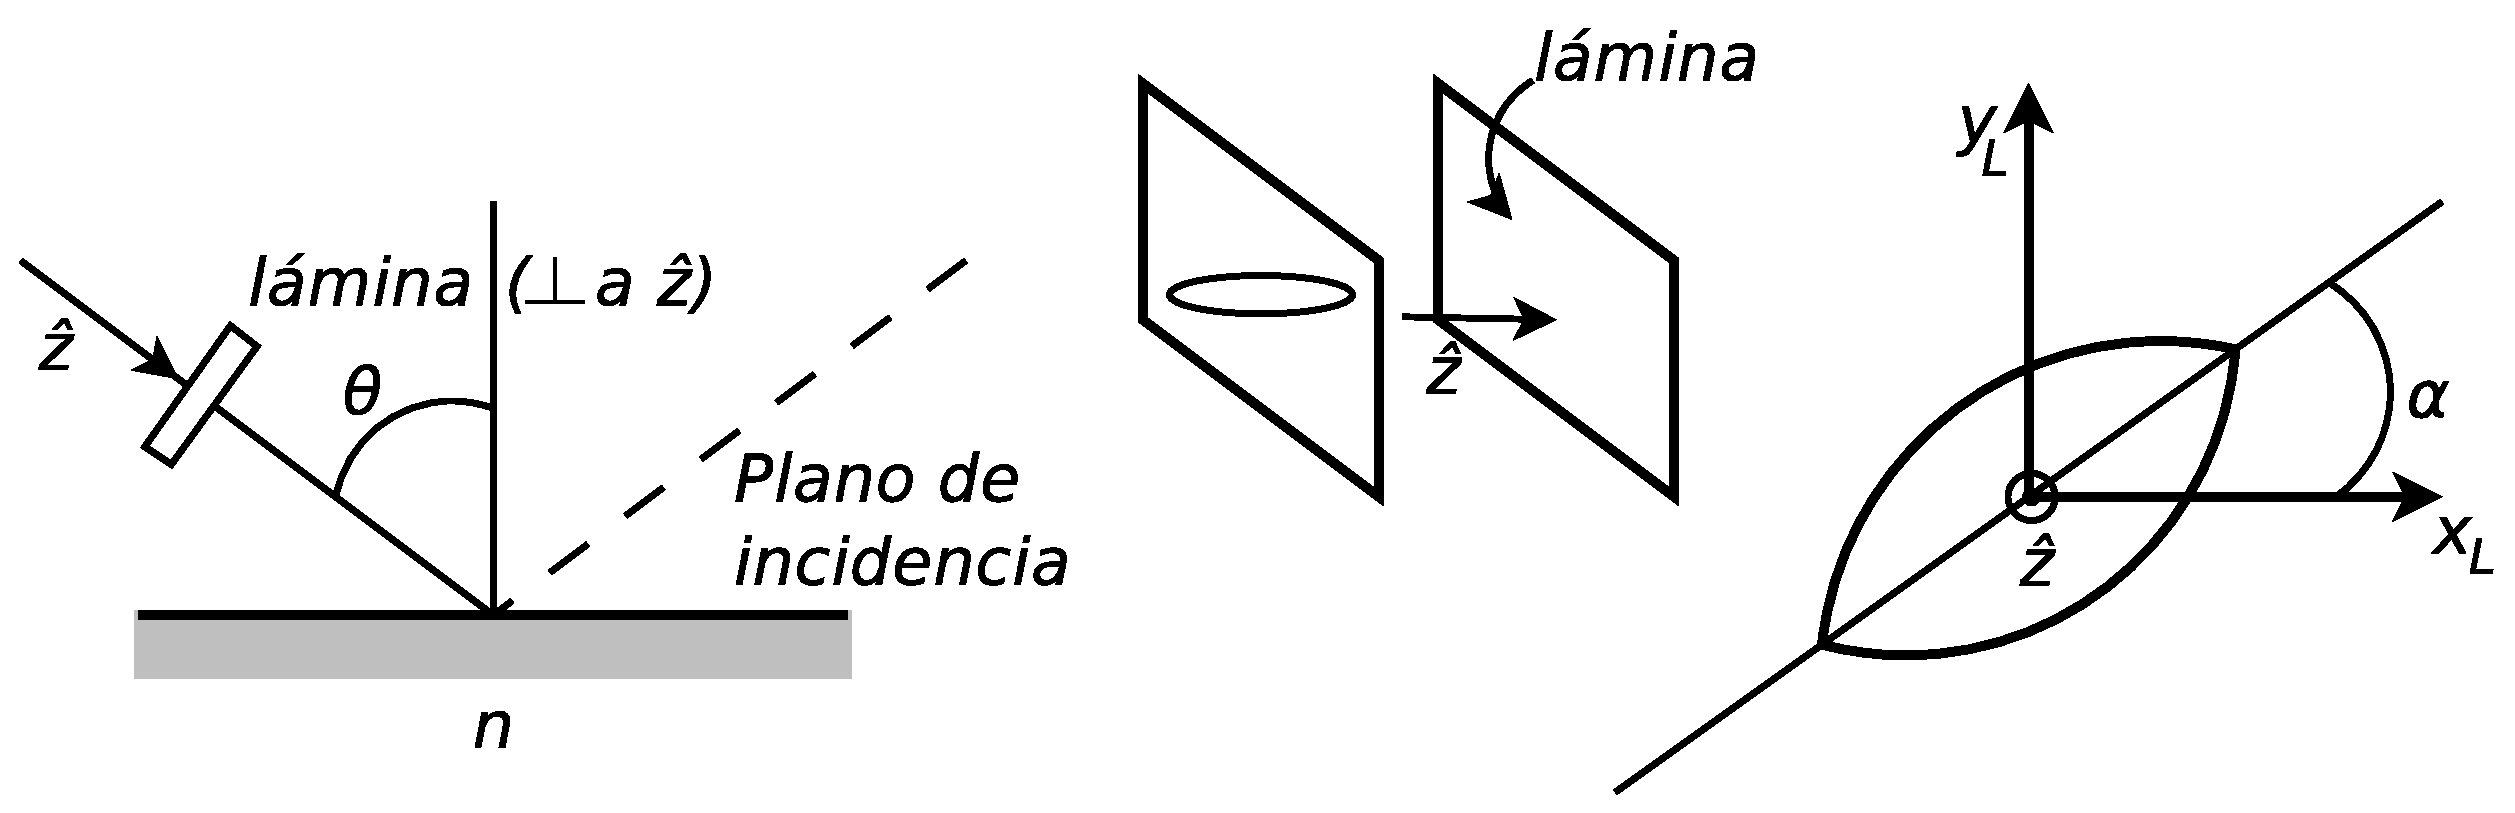
\includegraphics[clip,scale=0.25]{figs/ej4-28}
        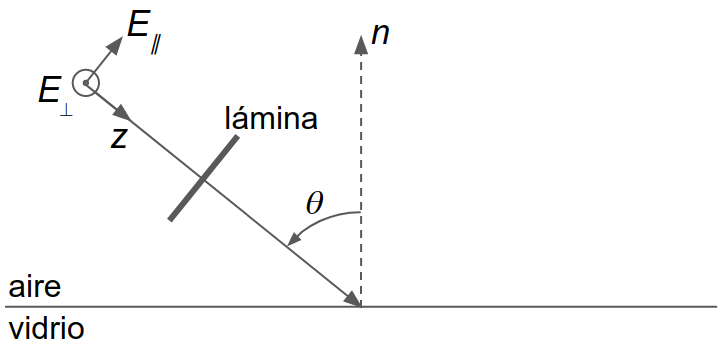
\includegraphics[clip,scale=0.45]{figs/brewster1.png}
    \end{figure}
    
    \begin{enumerate}
        \item ¿Cuánto debería valer el ángulo de incidencia $\theta$ para que
        pueda anularse la  onda reflejada? ¿Este requisito es condición
        suficiente?
        
        \item ¿Cuál debería ser la polarización del campo a la salida de la
        lámina?

        \item Determine cómo debe orientarse la fuente con respecto a los ejes
        de la lámina. Es decir, halle cuál debe ser el ángulo $\alpha$ formado
        entre el semieje menor de la elipse y el eje rápido de la lámina
        ($x_\text{L}$), para obtener la polarización deseada a la salida de la
        lámina.
        
        \item Halle el campo a la salida de la lámina, y determine el ángulo
        $\beta$ formado entre el eje $x_\text{L}$ de la lámina y la dirección
        perpendicular al plano de incidencia, para que dicho campo no tenga onda
        reflejada.
        
        \begin{figure}[H]
            \centering{}
            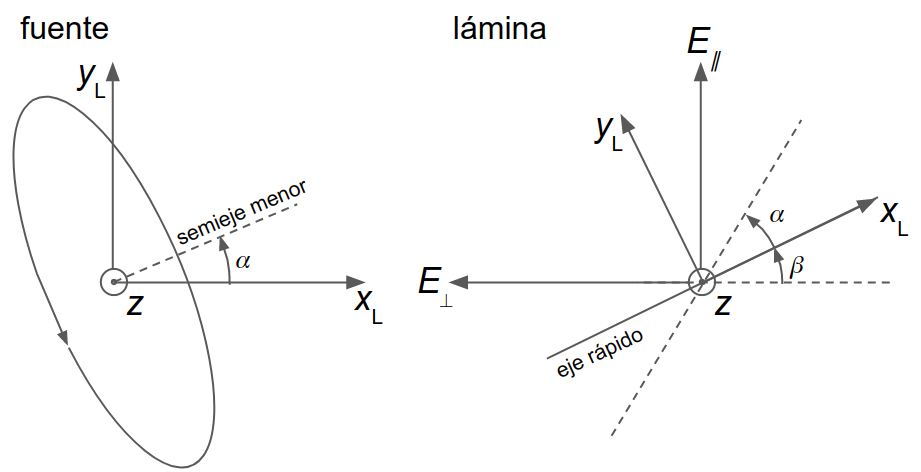
\includegraphics[clip,scale=0.45]{figs/brewster2.png}
        \end{figure}

    \end{enumerate}
    
    \textbf{Sugerencia:} escriba \textit{claramente} la expresión del campo
        eléctrico a la entrada y a la salida de la lámina, empleando (e
        indicando) diferentes sistemas de coordenadas si es necesario.
    
\end{enumerate}

\end{document}

